\subsection{Database Arkitektur}
\label{ssec: databaseArkitektur}
Systemets database vil stå for at opbevare data for brugerne, dette vil være i form af data indeholdt i et gemt spil.\\
I oprettelsen af systemets database skal der tages hånd om, hvordan kommunikationen skal foregå imellem systemets segmenter, samt databasens funktionalitet. Her er der blevet besluttet at der anvendes en DAL, der fungerer ved at hver gang databasen skal kontaktes, så foregår det igennem denne. Yderligere vil denne DAL også simplificere kommunikationen mellem databasen og Backend'en. 

\noindent Herunder vises et eksempel på hvordan kommunikationen ville foregå med databasen.

\begin{figure}[H]
\centering
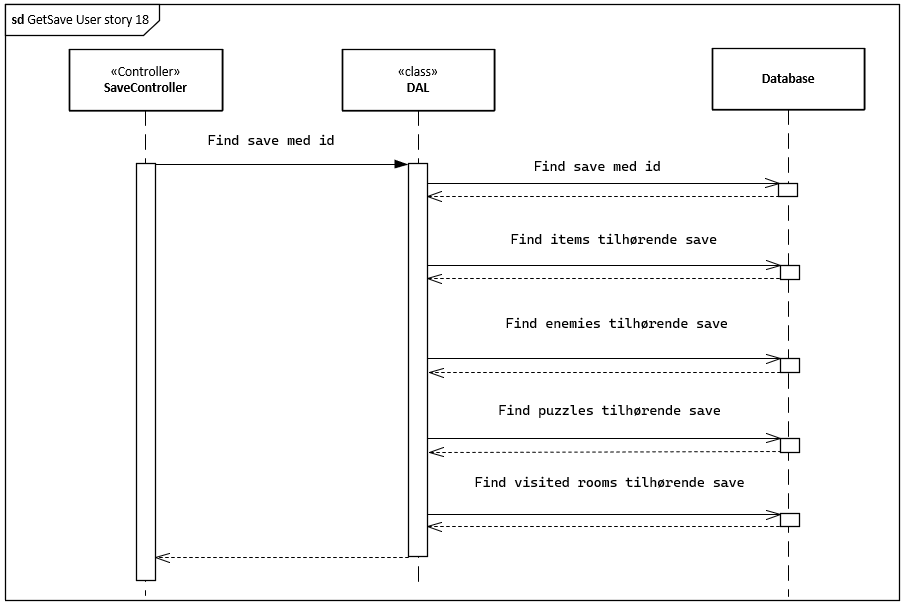
\includegraphics[width = \textwidth]{02-Body/Images/GetSaveDB.PNG}
\caption{Sekvensdiagram for User story 18: GetAllSaves, i relation til hentet data fra specifikt gemt spil fra database}
\label{fig:GetSaveDB}
\end{figure}

\noindent I figuren \autoref{fig:GetSaveDB} ses diagrammet GetSave, User story 18. Her ses der hvordan et specifikt gemt spil hentes. Her ses der at dataene igen går først igennem DAL. Et gemt spil vil have et ID, som der kan anvendes til at finde de korresponderende værdier som dette gemte spil har. Her ses der at der vil findes items, enemies, puzzles og hvilke rum en spiller har besøgt. Dataene returneres herefter til DAL og så til SaveController. Hvor det så kan anvendes videre i systemet.\\

\noindent Yderligere eksempler og forklaringer vedr. database arkitektur kan findes i teknisk bilag \parencite[][Section 9.5]{TekniskBilag}

\subsubsection{DAL Arkitektur}
Når data enten skal sendes til eller hentes fra databasen så er det igennem et DAL. Systemets DAL fungerer som en mellemmand for systemet, da alt kommunikation til og fra databasen går igennem den.\\
\noindent I dette DAL vil data for at gemme et spil og indlæse et spil blive sendt igennem. Begge af disse vil indeholde det samme type data, dog ville den ene, LoadGame, hente data fra systemets database, og den anden, SaveGame, vil sende data til systemets database. 
LoadGame, og SaveGame, i DAL vil være ansvarlig for at hente spillerens data fra databasen, såsom hvilket rum de var i og mængden af liv de har tilbage.\\

\noindent Yderligere eksempler og forklaringer vedr. DAL arkitektur kan findes i teknisk bilag \parencite[][Section 9.6]{TekniskBilag}
